\documentclass{article}
\usepackage[utf8]{inputenc}
\usepackage[ukrainian]{babel}
\PassOptionsToPackage{hyphens}{url}\usepackage{hyperref}
\title{Прикладні алгоритми. Завдання 3, звіт}
\author{Михайло Голуб}
\usepackage{graphicx}
\graphicspath{ {./images/} }
\begin{document}
\maketitle
\newpage

\textbf{Реалізація рекурсивного пошуку в глибину:}\\\indent

Рекурсивну функцію наведену в лекції "Топологічне сортування орграфів" було модифіковано наступним чином: замість помилки про знаходження циклу в графі, рекурсивна функція нічого не робить і повертається на попередній рівень рекурсії; замість обходу та перенумерації вершин -- визначення досяжності вершини з початкової.\\

\textbf{Реалізація алгоритму Уоршелла:}\\\indent

Алгоритм Уоршелла приймає на вхід граф та почергово обраховує часткові матриці досяжності доки не отримано матрицю досяжності всього графа. Якщо усі значення в матриці досяжності True -- граф зв'язний.\\

\textbf{Теоретична оцінка алгоритмів:}\\\indent

Рекурсивний пошук вглибину в найгіршому випадку (коли граф зв'язний) обійде всі ребра двічі, тож його складність в найгіршому випадку -- $O(e)$, де e -- кількість ребер. Максимальна кількість ребер в графі з v вершин -- $\frac{v(v-1)}{2}$. Отже, складність в найгіршому випадку -- O$(v^2)$. \\\indent
Алгоритм Уоршелла має складність $\Theta(v^3)$.

\textbf{Практична оцінка алгоритмів:}\\\indent

Для практичної оцінки алгоритмів створюється набір графів за заданними параметрами кількості вершин та ймовірності ребер, і на цьому наборі засікається час роботи алгоритмів. Для виключення впливу кешу процесора було проведено невеликі тести, які показали що порядок запуску алгоритмів не впливає на час роботи на однаковому графі.\\\indent
Нижче наведені результати тестів часу роботи рекурсивного пошуку в глибину та алгоритму Уоршелла:
\begin{center}
    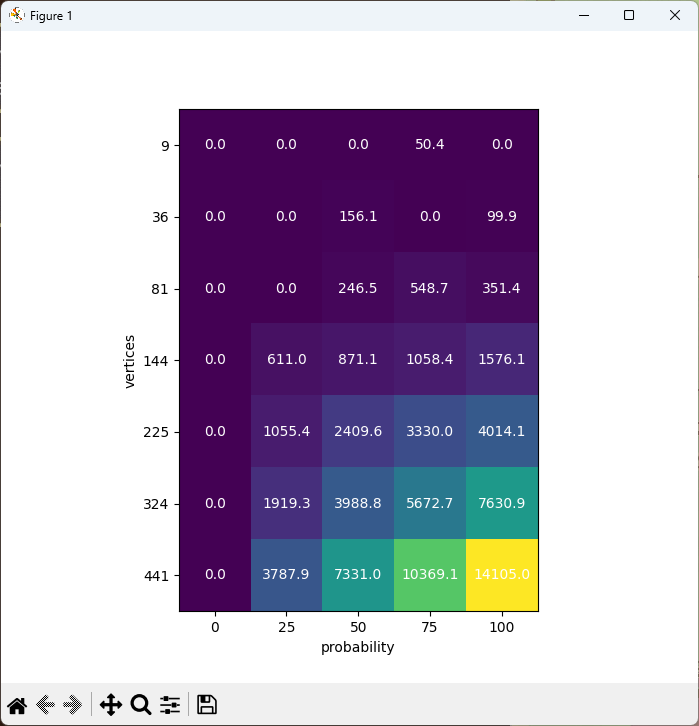
\includegraphics[width=125mm]{dfs_2}
    Час роботи рекурсивного пошуку в глибину
    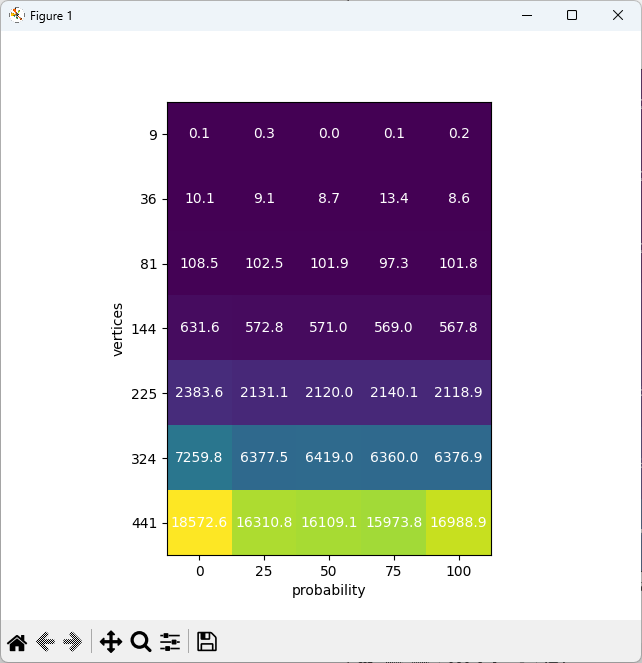
\includegraphics[width=125mm]{w_2}
    Час роботи алгоритму Уоршелла
\end{center}

З теплових карт видно, що:
\begin{itemize}
	\item Подвоєння ймовірності ребер призводить до приблизного подвоєння часу роботи рекурсивного пошуку в глибину;
	\item Явно існує кубічна залежність часу роботи алгоритму Уоршелла від кількості вершин;
	\item Час роботи алгоритму Уоршелла, з невідомих причин, більший в пустих графах;
	\item Якщо граф повний -- алгоритм Уоршелла швидший ніж рекурсивний пошук в глибину. Скоріше за все це пов'язано з тим, що рекурсивний пошук в глибину використовує повільні структури даних, а також велика частина часу йде на запуск рекурент.\\\indent
\end{itemize}

\textbf{Висновок:}\\\indent

Теоретична оцінка показує, що в найгіршому випадку рекурсивний пошук в глибину має бути швидшим ніж алгоритм Уоршелла. Проте, в цій реалізації, в найгіршому випадку рекурсивний пошук в глибину працює довше ніж алгоритм Уоршелла.

Посилання на репозиторій практикуму:\\ \href{$https://github.com/MINIAProgramStudio/applied_algorythms/tree/main/task_3$}{$https://github.com/MINIAProgramStudio/applied\_algorythms/tree/main/task\_3$}
\end{document}